%% note: todo's go in todo, as well as optionally in here

\section{Experiment Results}
For our initial experiments we first test how well our system scales under load. We download a small file (100KB) 
under different loads. In each test a given number of peers enter the system within 
the first 100s, using a poisson distribution with an inter arrival time that is 100s divided by the number of peers, 
so that they all enter pseudo-randomly within 100s. Peers start out by requesting the file from 
an origin server located on a well provisioned machine at BYU running an Apache2 web server that it 
bandwidth limited (using mod\_bw) to 256KB/s and 256 max connections. Peers are randomly selected from available PlanetLab 
hosts (a pool of up to 300 scattered world-wide on the PlanetLab system).  If more than 300 peers download the file,
then some PlanetLab hosts are re-used as proxies, though connections to other peers on the same computer
are disallowed.  Experiments run until 
all peers finish downloading the file. Each experiment is repeated 3 times and results are averaged. 
A different filename is downloaded each time, so as to use ``fresh" DHT keys with each run. We collect the download 
times of all peers, and measure the amount of load on the origin server by summing the bytes received within a given 
second from the origin\footnote{This only measures bytes received from the origin, not bytes sent, 
as any data received after a socket has already been closed are ignored, and peers 
close connections early if they receive the bytes from somewhere else}. We also calculate the percentage 
of the file received from peers versus from the origin, as well as the time required to do the DHT 
get, put, and remove operations during each run.  All box plots show 25th and 75th percentiles, with outlying lines showing
1st and 99th percentiles, and the middle-line showing the median.

We first test a traditional client-server transfer, to establish a base line from which to compare 
our system. Fig.~\ref{fig:client_server_download_times} shows the download times for client-server 
download, with various loads. Median download times have a low of 1.33s with 1 peer entering the system/second, 
and quickly grow up to a high of 344s at 20 peers/second. Download times increase linearly instead 
of exponentially because we start a fixed number of peers and let them all complete downloads, without more peers
entering the system. 
The top outliers at 20s are peers which typically waited in line about 900s before finally 
being served the file. Load on the origin server grew quickly to its theoretical cap of 250KB/s (Fig.~\ref{fig:client_server_server_load}) 
at 3 peers/s. Under higher load (20 peers/s), server speed actually decreases to 203KB/s, which 
shows the limitations of our bandwidth limiter in that it becomes bursty at higher connection rates. 

\begin{figure*}
  \begin{center}
    \subfigure[Load on the origin server]{
      \includegraphics[width=8cm]{pics/vr_unnamed316651_cs_stress_test/server_speed_Percentile_Line.pdf}
      \label{fig:client_server_server_load}
    }
    \subfigure[Download times]{
      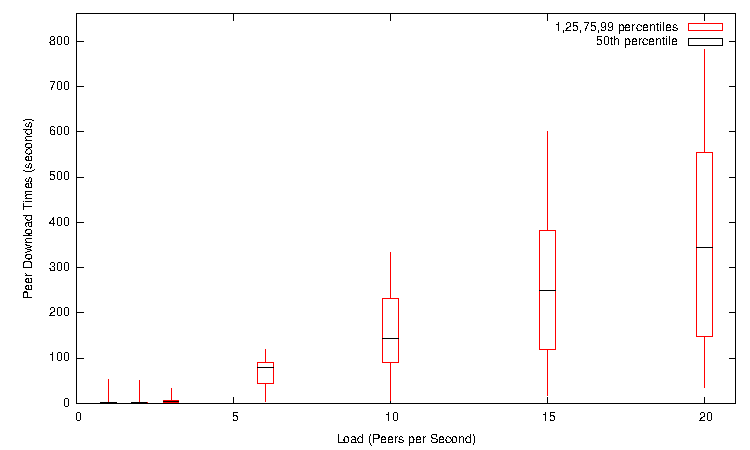
\includegraphics[width=8cm]{pics/vr_unnamed316651_cs_stress_test/client_download_Percentile_Line.pdf}
      \label{fig:client_server_download_times}      
    }     
    \caption{Traditional client server download}  
  \end{center}
\end{figure*}

We next test our system under the same loads. For default system parameters, we chose reasonable values 
of block size of 100KB, origin minimum speed (R) of 128KB/s, R's calculation window (W) 
of 2s, and first-byte timeout (T) of 1s. Peers linger, serving the file, for 20 seconds after completing 
a download, and download from up to 5 other peers at a time (b). Results for download median times 
(Fig. \ref{fig:yanc_download_times}) start at 1.4s with 1 peer entering the system/second, and grow 
to 5.23s at 6 peers/s and 7.46s at 20 peers/s. The graph's Y axis for download time (Fig. \ref{fig:yanc_download_times}) 
is different than that for client-server (Fig.~\ref{fig:client_server_download_times}, above) 
because the difference is so great that it would obscure the details. At a load of 20 peers/s 99.5\% 
of peers give up on the origin server because of a slow first byte (T) after one second. They then query the 
DHT for a peer list, and receive a response with a median latency of 5.215s.  They download the file almost 
immediately once they receive their peer list, hence the median of about 7s. Of those that took longer 
there are two basic causes. One is that poorly connected peers take so long to download a file 
that the linger times of peers they request the file from begin to expire (and the connection is dropped).   They then have to request a new 
list of peers, causing a repeat in latency.  This problem is exacerbated by the fact that we request 
the last block from multiple peers, in order to try to avoid a slow last block problem.  This causes 
redundancy in bytes received, which slows down slow peers, causing them to timeout peer 
connections even more often. The other factor causing slowdown is a sometimes unresponsive DHT. We 
set DHT requests to timeout after 60s if no response was received--a reasonable value to keep from 
overloading the DHT. Typically requests came back quickly, however at times they would timeout, 
and peers would end up downloading the entire file from an (overloaded) origin, or perform a new 
query after 60s, and then quickly download the file after that.  We're not entirely sure why this behavior occurs with Pastry.
The amount received from the origin decreases with higher load, mostly because mod\_bw serves 
very little when it is under high load, but also because the peers receive the file much more quickly 
from their peers so abandon their connections to the origin (Fig. \ref{fig:yanc_origin_server_load}). 
<%= figure_directory 'vr_medium_p2p_load_tak4', 'yanc', 'P2P results varying load' %>

The amount of peer-to-peer transfer, as expected, increases with higher loads. Under low load peers tend to download 
the file only from the origin, however, after about 10 peers/s almost 100\% of the transfer is being 
done from peers (Fig.~\ref{fig:yanc_cdf_from_peers}--a 1 on the graph means 100\% of the file 
transfer is from peers). The reason it isn't always at 100\% for lower loads is that peers start 
downloading the file from the origin, receive some portion of it within the first $W$ (2) seconds, 
transition to peer-to-peer transfer because the rate of download is less than $R$, then receive the rest from their peers. 
The 1st percentile almost always download the entire file from the origin 
(typically the first few peers to enter the system), while later peers almost always download the 
file from their peers, because they encounter a slow origin server. 
\section{Impact of various parameters}

Theoretically, if a peer can download a file quickly from the origin, it does not benefit it to download the file also from its
peers. Our system accomodates for this by specifying parameters for the conditions under which it will 
transition to a peer-to-peer delivery. We next test the impact of varying these and other parameters, in order 
to explore the dynamics of our system. In each test we run 1000 peers, with an average of 15 peers entering 
the system per second, using a poisson distribution with an interarrival time of 0.066s (peers enter the system within 67s). 
We then wait for all peers to finish downloading. They download a 100KB file, use a default block size of 100KB, and a 20 peer
connection limit ($b$). $T$ is set by default to 1s, $R$ to 128KB/s, and $W$ to 2s. 

\subsection{Time to wait for first byte T}

We first vary $T$, the timeout for a first response byte from the origin server. We expect that an extremely low value 
will cause transitioning too early and an extremely high value 
will cause transitioning too late, both resulting in slower download times. The results held to our hypothesis for low values but not for 
high. With a $T$ setting of 0s, median download time is 12s. It then drops to 4.5s with $T$ set at 0.75s, 
rises to 10s with $T$ set at 2s, and flattens out for higher values than 2 (Fig. \ref{fig:vary_t_download_times}). 
The reason it flattens out, instead of increasing as we expected, is that T's relative importance decreases when it 
is set too high, and $R$ causes the transition more often.  

Fig. \ref{fig:vary_t_death_reasons} shows the different transition causes that caused peers to transition to peer-to-peer delivery.  dT is the number
of peers who transition to peer-to-peer delivery because of a slow first byte, dR is the number of
peers that transition because of a too low value of R, died is the number of peers that never completed the download
(typically because their host's network access had connectivity problems) and http\_straight refers to the number of peers
that downloaded the entire file from the origin server.

With low values of $T$, almost 100\% of peers transition to peer-to-peer delivery because of $T$. With $T$ set at 10s
about 80\% of peers transition because of $T$, and 20\% because of $R$, so a higher value of $T$ didn't cause a slowdown, it
just caused $R$ to become more important, and the transition to peer-to-peer delivery still occurred.
%The outliers for download time are usually peers who were poorly connected to the DHT, so they sometimes 
%received answers to their queries after the answers were already outdated, so had trouble connecting 
%to live peers. 
<%= figure_directory 'vr_unnamed17712_dT', 'vary_t', 'Varying T', true, false %>

\subsection{Server minimum allowed speed R}

We next examine the effect of varying $R$, the server's minimum allowable speed.  This value is calculated 
by peers summing the number of bytes received from the origin over the previous $W$ seconds. We vary $R$ from 32KB/s to 1MB/s, and leave $T$ set to a 
reasonably high value of 10s and $W$ set to 2s. The expected result us that a high value of $R$ would cause transition 
too early, and that a value too low would cause transition too late, both resulting in poor performance. This was the case.  With $R$ set 
to 5KBps, median download times are 40s, with $R$ at 40KBps, download times dropped to 15s, and reached 
a low of 13s with $R$ set to 160KBps. $R$ set to 1MBps has a median download time of 30s (Fig.~\ref{fig:vary_dr_download_times}). 
<%= figure_directory 'vr_unnamed502788_dR_fromStart_5000by_fixed_settingAndMajorTimes_8_times_0.0666666666666667s__10s_100000B_255000BPS_5000s_10s_2.0s_100000B', 
  'vary_dr', 'Varying R', false, false %> 

\subsection{Server speed time window W}

We next vary $W$, the amount of recent download time used to calculate $R$. Our hypothesis is that 
a small value for $W$ will cause calculation to be too sensitive and unoptimal. We vary $W$ from 0.1s 
to 10s and run the experiment described above (for $R$) with $T$ set to 10s and $R$ set to 128KB/s. The results are 
slightly different than our hypothesis. Varying $W$ does make some difference, but only when set 
to a very low value. Median download times are 17s with $W$ set to 0.25s. For $W$ \textgreater{} 0.25s 
median download times stayed at around 25s (Fig.~\ref{fig:dw_download_times}). Surprisingly, 
most peers (consistently about 800 out of 1000) still transition to peer-to-peer delivery because of 
a slow first byte ($T$), even with $T$ set to the larger value of 10s (Fig.~\ref{fig:dw_death_reasons}). 
The reason for this is that we don't start calculating $R$ until after the first byte is received, and 
in the majority of cases (800/1000) this didn't happen until after $T$ had expired, at 10s, so $T$ still 
causes most of the transitioning. A lower value of $W$ only affected the first 
200 peers, who do receive bytes from the origin, causing them to transition more quickly to peer-to-peer delivery.

% ltodo so was it all the first 200 that always transition to R, so that's what sped things up a bit?

% why was this higher, then?

<%= figure_directory '837145_dw', 'dw', 'Varying W', true, false %>

\section{Effect for a full web page}

We next run an experiment more indicative of real-world web page. The normal pattern for a page view 
is to first access some root page which references several others, such as images, 
javascript, flash, etc. This is the case for the BYU web site, which has a medium sized main page that 
links to over 10 small other objects\footnote{ Snapshot 2007}. We therefore next run an experiment 
to see how well our system downloads a small page followed by several smaller files. Each peer first 
downloads a 100K file. When that file completes each peer then downloads 10 10K files simultaneously 
(all from the origin server), and the total time to download all 11 files is measured. We set the parameters 
to be those mentioned above for varying $R$, varying the incoming speed of peers from 1 peer/s to 25 peers/s. 
The expected result is that downloading multiple pages will be slower than downloading only one 
since it will put more stress on the DHT, which proved correct (Fig. \ref{fig:multiple_files_download_times_all_files}). 
Total download time starts at 1.3s, and appears to grow dramatically with increased load, approaching 
150s at 25 peers/s. DHT response times also grow with load, starting 
at a median of 0.41s at 1 peer/s for put queries, and growing to a median of 12s/query at 25 peers/s 
(Fig. \ref{fig:multiple_files_p2p_dht_put}). This causes quite a bit of slowdown because our
linger time is set to 20s, so peer lists become outdated soon after they are created.  Also interesting to note is 
the load on the origin server (Fig. \ref{fig:multiple_files_origin_server_load}), which goes down when there are 
 10 peers per second (most of the download is being down from peers), but, at higher loads than this, increases as our 
system is not able to handle the strain of more peers.

% todo is that what really happens though?

\begin{figure*}\begin{center} 
 \subfigure[Download times] {
  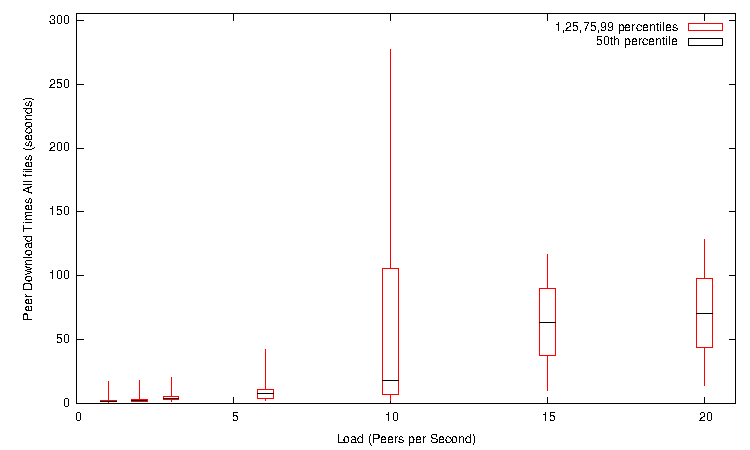
\includegraphics[width=8cm,]{pics/vr_multiples_take_1/client_download_all_files_Percentile_Line.pdf}
  \label{fig:multiple_files_download_times_all_files}
 } 
 \subfigure[Load on the origin server] {
  \includegraphics[width=8cm,]{pics/vr_multiples_take_1/server_speed_Percentile_Line.pdf}
  \label{fig:multiple_files_origin_server_load}
 } 
 \subfigure[Percent of file received from peers] {
  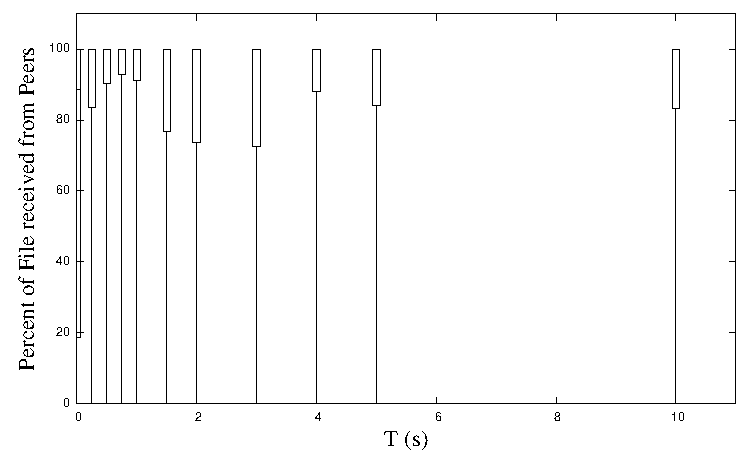
\includegraphics[width=8cm,]{pics/vr_multiples_take_1/percent_from_clients_Percentile_Line.pdf}
  \label{fig:multiple_files_cdf_from_peers}
 }
 \subfigure[DHT put times] {
  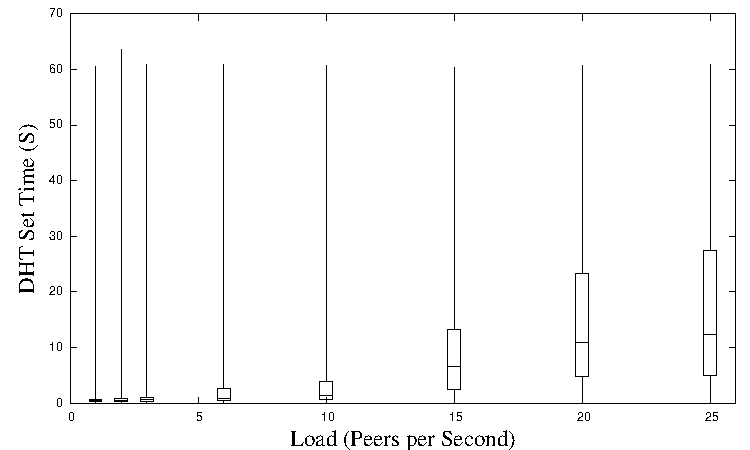
\includegraphics[width=8cm,]{pics/vr_multiples_take_1/dht_Put_Percentile_Line.pdf}  
  \label{fig:multiple_files_p2p_dht_put}
 }
    \caption[]{Downloading multiple simultaneous files}
    \end{center}
    \end{figure*}

We next re-run the same test using a traditional client-server download. Download times using 
client-server grew at a much steeper rate (Fig. \ref{fig:multiple_files_cs_download_times}). 

<%= figure 'pics/multiples_p2p_versus_cs_pics/client_download_Percentile_Line.pdf', :caption => 'Comparison of P2P versus client server download times for multiple files', :label => 'fig:multiple_files_cs_download_times' %> 

\subsection{Varying Block Size}

We next measure the effect block size has on download time. We download a 100K file with block sizes from 
16KB to 100KB. We run 1000 peers at an average of 15 peers entering per second. 32K blocks resulted 
in the quickest downloads (a 10.6s median) (Fig.~\ref{fig:vary_block_size_download_times}), because our system
allowed itself to download different bytes from several different peers, per file.

%32KB blocks were shown to be effective in \cite{TODO}.  

<%= figure_directory 'vr_unnamed240998_blockSize', 'vary_block_size', 'Varying block size', false, false %>

\section{Downloading Large Files}

We next test our system's ability to download large files. We download a 30MB file with 100 peers, 
and then download the same file, using BitTorrent with similar 
settings. Block size is set to 256K for both systems. Peers enter the system at an average of 1/s, 
and both protocols' origin servers are rate limited to 256KB/s. For both systems, peer linger time 
is set to 0s (though peers still share the file while they are downloading it). 
The expected result is that the two fare similarly. It turns out that a few peers download 
faster with our system, but most download faster with BitTorrent (Table~\ref{fig:yanc_vs_bt}). 
Ours had a slower median than BitTorrent (847s to 148s), though BitTorrent was worse for the 99th 
percentile (2786s to 847s). We're not entirely sure exactly which factors make BitTorrent faster.
We know of a few differences that could make a difference.  One is that BitTorrent's seed limits its number of outgoing connections
to 7 (Apache--our server--does too, but to 256). This enables BitTorrent to propagate blocks more 
quickly to peers, who then spread the blocks out to other peers. BitTorrent seeds also favor peers who have higher download 
speeds, which helps speed propagation. BitTorrent in this test uses a dedicated tracker, 
which also made peer rendezvous quicker than using our DHT.  It uses a ``rarest block first" policy in block 
selection, enabling it to share blocks more efficiently.  These differences combined allow it 
to respond to a flash crowd such as this one better.  In future work we will optimize our system to handle 
flash crowds such as this one.  One interesting statistic is the relative download percentiles. 
The difference between 25th and 75th percentiles of our system is about 150s, 
or 5\% of the 75th percentile's time. The difference between the 25th and 75th percentiles of BitTorrent 
is 24s, or about 7\% of the 75th percentile's time. These numbers being similar means that once 
a few peers have downloaded the file, it doesn't take (relatively) long in either system for the rest of the peers to complete 
the download (Fig.~\ref{fig:yanc_30mb_cdf}). Very few peers receive more than 50\% of the file 
from the origin (2\%). 

<%= figure 'pics/yanc_30mb/yanc_30_mb_cdf.pdf', :caption => 'CDF of percent of file received from peers, 30MB file', :label => 'fig:yanc_30mb_cdf' %>

\begin{table}
  \caption{Download times of a 30MB file}
\begin{tabular}{ c c l }
  Percentiles & Our System (S) & BitTorrent (S) \\
  \hline
  1 & 613 & 131 \\
  25 & 730 & 139 \\
  50 & 847 & 148 \\
  75 & 882 & 163 \\
  99 & 982 & 2786 \\
  \label{fig:yanc_vs_bt}
\end{tabular}
\end{table}
  
\section{Peer connection limit b} 

We next vary the maximum number of download connections each peer is allowed to have at a time ($b$). We 
repeat the above (30 MB file) experiment using our system, and vary the peer connection limit from 1 to 50. 
We expect that download times will suffer if the connection limit is too low. As expected, median 
download times suffered with a low limit, with a mediain download time of 1604s with limit 1. Download 
times decreased with a higher connection limit, with 16 yielding a median download time of 931s 
(Fig. \ref{fig:vary_connection_count_download_times}).  Limits greater than 16 didn't 
yield as much relative gain. A 50 peer limit resulted in a median download time of 875s.

<%= figure_directory 'vr_vary_blocks_large_file', 'vary_connection_count', 'Varying number of concurrent peers', false, false %>

\section{Varying linger time}

We next vary the amount of (post file download) linger time, our hypothesis being that a longer linger 
time will increase download speeds, which proved correct (Fig.~\ref{fig:vary_linger_time_download_times}). 
We download a 100K file (using the same parameters as the original $R$ test) varying linger time. The 
results confirm our hypothesis. With a linger time of 0s, median download time was near 300s, with 
a median download time of 127s with linger time at 1s, 60s with linger 2s, 34s with linger time of 4s, 
and staying mostly constant for linger times greater than 4s near 30s.

<%= figure_directory 'vr_unnamed497104_linger_fromStart_0by_fixed_settingAndMajorTimes_8_times_0.0666666666666667s__0s_100000B_255000BPS_125000s_1.0s_2.0s_100000B', 
 'vary_linger_time', 'Varying linger time', false, false %> 
